\section{Preliminaries}
\label{sec:preliminaries}
In this section, we provide some background on Ethereum and its account model. For a deeper dive into Ethereum, we refer the reader to~\cite{antonopoulos2018mastering}. Moreover, we briefly describe the high-level workings of Tornado Cash.

\subsection{Ethereum and the Account Model}
Ethereum is the second-largest cryptocurrency platform in terms of market capitalization.\footnote{For more details, see: \url{https://coinmarketcap.com/currencies/ethereum}.} However, it is the largest smart contract platform, and it is also the most used public blockchain for settling transactions. Therefore, it is imperative to understand better and assess the privacy guarantees of Ethereum quantitatively.

Ethereum employs the \textit{account model}. There are two types of accounts: externally owned accounts (EOA) and contract accounts. EOAs are controlled by users via a cryptographic key-pair (a private and a public key) owned by them. The private key of the EOA enables users to send transactions from that account, while the public key is used to derive an address for the EOA (the hash of the public key is its address). On the other hand, contract accounts are controlled by contract code. The contract account's address is the hash of their contract code. Accounts are referred to by their addresses (a pseudonym). Contract accounts cannot initiate transactions. However, EOAs can send transactions to contract accounts that can run the code of the contract account. In the following, we will use the words accounts and addresses interchangeably. 

% mw: took out bc we don't really use this
% All accounts have the following fields:
% \begin{itemize}
%     \item \textbf{Balance:} it denotes the amount of ether (the native currency of the Ethereum blockchain) the account owns.
%     \item \textbf{Nonce:} the number of confirmed transactions the account has sent. This field facilitates the prevention of replay attacks. For instance, the receiver of a transaction cannot drain the sender's balance by replaying transactions since transactions also sign off the nonce field of the sender's account.
%     \item \textbf{Storage:} it is a permanent data store for account contracts. This field is empty for EOAs.
%     \item \textbf{Code:} only contract accounts possess code, EOAs do not.
% \end{itemize}

Ethereum's account model has several implications from a privacy point of view. First, the account model incentivizes the reuse of accounts across many transactions. Imagine the following scenario. Alice owns an EOA with address A and a balance of three ether. Alice wishes to buy a product from Bob for two ether. Alice sends a transaction worth two ether to Bob. After this purchase, address A has a balance of one ether. Therefore, if Alice wants to spend her change, she necessarily needs to send a transaction \emph{again} from her address A. Address reuse facilitates the profiling of rich transaction histories: complete financial history,  list of all counterparties, time-of-day activity, and more. Furthermore, account reuse implies that most users only own a handful of accounts. Finally, the accounts owned by the same user can effectively be clustered; see Section~\ref{sec:eth}. 

\subsection{Preserving Privacy on Ethereum: Tornado Cash}
Users can break links with their transaction history using a so-called mixer contract. Tornado Cash (TC) is the most widely used, non-custodial mixer on Ethereum. TC works as follows. Users deposit equal amounts to a TC smart contract (e.g. 1 ETH as shown below). After some time, users can withdraw their funds from the mixer contract to \emph{a freshly generated EOA} by providing a zero-knowledge proof that proves that the withdrawing user is one of the depositors. Therefore, the withdrawing EOA has enhanced its privacy since it has become unlinkable to any unique depositor EOA. Note that each TC contract applies a fixed denomination for the mixed funds (e.g. 1 ETH). Otherwise, linking deposits to withdraws would be trivial.

\begin{figure}[h!]
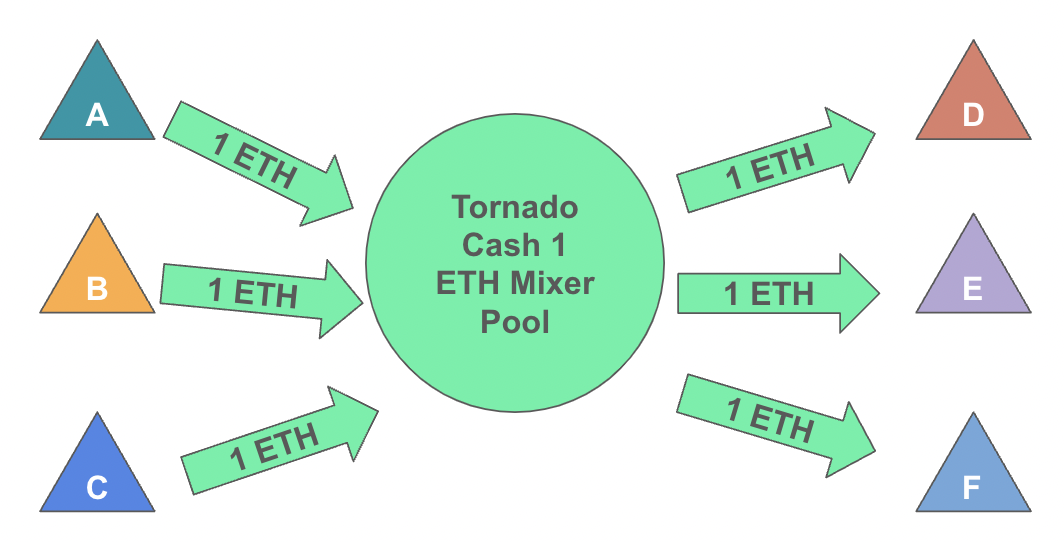
\includegraphics[width=\linewidth]{figures/Mixer_WW.png}
\caption{Example of the Tornado Cash 1 ETH pool: addresses A through F deposit to and withdraw from the pool. It quickly becomes impossible to associate withdraw and deposit transactions given a growing mixer.}
% \istvan{This figure is too small, I'm afraid.}
% \mike{is this better?}
\label{fig:demo}
\end{figure}

A user's anonymity is defined by the number of equal user deposits in a given pool. This is the pool's \emph{Anonymity Set}. In the example above, D’s withdrawal could have come from A, B or C, so the anonymity set is 3 and the probability of correctly guessing the deposit / withdrawal connection is 1/3.

The more users that deposit in the pool, the greater the number of people that a withdrawal could have come from. If you add a fourth deposit to the example above, the probability of being correctly detected decreases to 1/4.
However, there are lots of ways users can compromise their privacy. If you can link A’s deposit to E’s withdrawal, then the pool’s anonymity set decreases from 3 to 2. This means the probability of correctly guessing your deposit / withdrawal connection increases to 1/2 because any withdrawal could only have come from B or C’s deposits.

Tornado Cash provides mixing contracts (otherwise known as mixing pools) for Ether and several Ethereum-based tokens (e.g., DAI, USDC, wBTC, etc.) in different denominations (1, 10, 100, etc.).
